\documentclass{beamer}
\usetheme{Frankfurt}
\addtobeamertemplate{navigation symbols}{}{%
    \usebeamerfont{footline}%
    \usebeamercolor[fg]{footline}%
    \hspace{1em}%
    \insertframenumber/\inserttotalframenumber
}

\usepackage{mathtools}
\usepackage{graphicx}
\usepackage{braket}
\usepackage{amsthm}
\usepackage{lmodern}
\usepackage[utf8]{inputenc}
\usepackage[frenchb]{babel}
\usepackage[T1]{fontenc}
\usepackage{subcaption}
\usepackage{caption}
\usepackage{gensymb}
\usepackage{tikz}
\usepackage[qm]{qcircuit}
\usepackage{listings}
\usepackage{pgfplots}
\usepackage{xcolor}
\usepackage{amsmath}
\usepackage{color, colortbl,booktabs}
\usepackage[ruled,vlined]{algorithm2e}
\captionsetup[figure]{labelformat=empty}

\definecolor{mGreen}{rgb}{0,0.6,0}
\definecolor{mGray}{rgb}{0.5,0.5,0.5}
\definecolor{mPurple}{rgb}{0.58,0,0.82}
\definecolor{backgroundColour}{rgb}{0.95,0.95,0.92}
\definecolor{Gray}{gray}{0.9}
\lstdefinestyle{CStyle}{
    backgroundcolor=\color{backgroundColour},   
    commentstyle=\color{mGreen},
    keywordstyle=\color{magenta},
    numberstyle=\tiny\color{mGray},
    stringstyle=\color{mPurple},
    basicstyle=\footnotesize,
    breakatwhitespace=false,         
    breaklines=true,                 
    captionpos=b,                    
    keepspaces=true,                 
    numbers=left,                    
    numbersep=5pt,                  
    showspaces=false,                
    showstringspaces=false,
    showtabs=false,                  
    tabsize=2,
    language=Python
}

\begin{document}
\section[Construction de circuits]{Construction de circuits}

\begin{frame}
    \frametitle{Portes \texttt{CNOT}}

    \begin{block}{Porte de Pauli X contrôlée par $n$ qubits }

        On note le contrôle par 1 avec $\bullet$ (le qubit de sortie $\ket{x_3}$ vaut 1 quant le qubit de contrôle vaut 1);

        On note le contrôle par 0 avec $\circ$ (le qubit de sortie $\ket{x_3}$ vaut 1 quant le qubit de contrôle vaut 0).

        Le contrôle global est un \texttt{ET} des contrôles individuels.

    \end{block}
    \begin{block}{Exemple}
        \begin{figure}[H]
            \centering
            \centerline{
                \Qcircuit @C=1em @R=.7em {
                    \lstick{ \ket{x_0}  } & \ctrlo{1} & \qw & \qw\\
                    \lstick{ \ket{x_1}  } & \ctrl{1} & \qw & \qw\\
                    \lstick{ \ket{x_2}  } & \ctrlo{1} & \qw & \qw\\
                    \lstick{ \ket{x_3} } & \targ\qw & \qw & \qw\\
                }
            }
            \caption{$\ket{x_0, x_1, x_2, x_3} \mapsto \ket{x_0, x_1, x_2, x_3 \oplus (\neg x_1 \land x_2 \land \neg x_3) }$}
            \label{fig:basic_control}
        \end{figure}
    \end{block}

\end{frame}

\begin{frame}
    \frametitle{Construction du circuit}

    \only<1>{
    \begin{block}{4 étapes de compilation}
        \begin{enumerate}
            \item \'Ecriture de la table de vérité,
            \item Pour chaque sortie donnant 1, former une porte \texttt{NOT} controlée. Chaque entrée va servir de contrôle, par 1 si l’entrée est à 1, et par 0 si l’entrée est à 0,
            \item Développement du circuit pour n'avoir que des portes \texttt{NOT} contrôlées par 0,
            \item Simplification du circuit.
        \end{enumerate}
    \end{block}
    }

    \only<2, 3, 4, 5>{
    \begin{columns}
        \begin{column}{0.5\textwidth}
            \begin{block}{Exemple}
                Soit la fonction booléenne $f(x_1, x_2, x_3) = (x_1 \land x_2) \lor (x_3 \land \neg x_2) \lor (x_1 \land x_3)$.
                \only<2>{
                    \begin{table}[!htbp]
                        \centering
                        \begin{tabular}{|c c c |c |}
                            \hline
                            $x_1$ & $x_2$ & $x_3$ & F($x_1$, $x_2$, $x_3$)\\ \hline
                            0 & 0 & 0 & 0 \\
                            0 & 0 & 1 & 1 \\
                            0 & 1 & 0 & 0 \\
                            0 & 1 & 1 & 0 \\
                            1 & 0 & 0 & 0 \\
                            1 & 0 & 1 & 1 \\
                            1 & 1 & 0 & 1 \\
                            1 & 1 & 1 & 1 \\ \hline
                        \end{tabular}
                    \end{table}
                }
                \only<3>{
                    \begin{table}[!htbp]
                        \centering
                        \begin{tabular}{|c c c |c |}
                            \hline
                            $x_1$ & $x_2$ & $x_3$ & F($x_1$, $x_2$, $x_3$)\\ \hline
                            0 & 0 & 0 & 0 \\
                            \rowcolor{mGreen}
                            0 & 0 & 1 & 1 \\
                            0 & 1 & 0 & 0 \\
                            0 & 1 & 1 & 0 \\
                            1 & 0 & 0 & 0 \\
                            1 & 0 & 1 & 1 \\
                            1 & 1 & 0 & 1 \\
                            1 & 1 & 1 & 1 \\ \hline
                        \end{tabular}
                    \end{table}
                }
                \only<4>{
                    \begin{table}[!htbp]
                        \centering
                        \begin{tabular}{|c c c |c |}
                            \hline
                            $x_1$ & $x_2$ & $x_3$ & F($x_1$, $x_2$, $x_3$)\\ \hline
                            0 & 0 & 0 & 0 \\
                            \rowcolor{mGreen}
                            0 & 0 & 1 & 1 \\
                            0 & 1 & 0 & 0 \\
                            0 & 1 & 1 & 0 \\
                            1 & 0 & 0 & 0 \\
                            \rowcolor{mGreen}
                            1 & 0 & 1 & 1 \\
                            1 & 1 & 0 & 1 \\
                            1 & 1 & 1 & 1 \\ \hline
                        \end{tabular}
                    \end{table}
                }
                \only<5>{
                    \begin{table}[!htbp]
                        \centering
                        \begin{tabular}{|c c c |c |}
                            \hline
                            $x_1$ & $x_2$ & $x_3$ & F($x_1$, $x_2$, $x_3$)\\ \hline
                            0 & 0 & 0 & 0 \\
                            \rowcolor{mGreen}
                            0 & 0 & 1 & 1 \\
                            0 & 1 & 0 & 0 \\
                            0 & 1 & 1 & 0 \\
                            1 & 0 & 0 & 0 \\
                            \rowcolor{mGreen}
                            1 & 0 & 1 & 1 \\
                            \rowcolor{mGreen}
                            1 & 1 & 0 & 1 \\
                            \rowcolor{mGreen}
                            1 & 1 & 1 & 1 \\ \hline
                        \end{tabular}
                    \end{table}
                }
            \end{block}
        \end{column}
        \begin{column}{0.5\textwidth}
            \only<2>{
            \begin{figure}[H]
                \centering
                \centerline{
                    \Qcircuit @C=1em @R=.7em {
                        \lstick{ \ket{x_1}} & \qw & \qw\\
                        \lstick{ \ket{x_2}} & \qw & \qw\\
                        \lstick{ \ket{x_3}} & \qw & \qw\\
                        \lstick{ \ket{x_f}} & \qw & \qw\\
                    }
                }
                \caption{Circuit quantique pour $f(x_1, x_2, x_3)$}
                \label{fig:circ_ex_1_1_6}
            \end{figure}
            }
            \only<3>{
                \begin{figure}[H]
                    \centering
                    \centerline{
                        \Qcircuit @C=1em @R=.7em {
                            \lstick{ \ket{x_1}} & \ctrlo{1} & \qw & \qw\\
                            \lstick{ \ket{x_2}} & \ctrlo{1} & \qw & \qw\\
                            \lstick{ \ket{x_3}} & \ctrl{1}  & \qw & \qw\\
                            \lstick{ \ket{x_f}} & \targ\qw  & \qw & \qw\\
                        }
                    }
                    \caption{Circuit quantique pour $f(x_1, x_2, x_3)$}
                    \label{fig:circ_ex_1_2}
                \end{figure}
            }
            \only<4>{
                \begin{figure}[H]
                    \centering
                    \centerline{
                        \Qcircuit @C=1em @R=.7em {
                            \lstick{ \ket{x_1}} & \ctrlo{1} & \ctrl{1} & \qw & \qw\\
                            \lstick{ \ket{x_2}} & \ctrlo{1} & \ctrlo{1} & \qw & \qw\\
                            \lstick{ \ket{x_3}} & \ctrl{1} & \ctrl{1} & \qw & \qw\\
                            \lstick{ \ket{x_f}} & \targ\qw & \targ\qw & \qw & \qw\\
                        }
                    }
                    \caption{Circuit quantique pour $f(x_1, x_2, x_3)$}
                    \label{fig:circ_ex_1_3}
                \end{figure}
            }
            \only<5>{
                \begin{figure}[H]
                    \centering
                    \centerline{
                        \Qcircuit @C=1em @R=.7em {
                            \lstick{ \ket{x_1}} & \ctrlo{1} & \ctrl{1} & \ctrl{1} & \ctrl{1} & \qw & \qw\\
                            \lstick{ \ket{x_2}} & \ctrlo{1} & \ctrlo{1} & \ctrl{1} & \ctrl{1} & \qw & \qw\\
                            \lstick{ \ket{x_3}} & \ctrl{1} & \ctrl{1} & \ctrlo{1} & \ctrl{1} & \qw & \qw\\
                            \lstick{ \ket{x_f}} & \targ\qw & \targ\qw & \targ\qw & \targ\qw & \qw & \qw\\
                        }
                    }
                    \caption{Circuit quantique pour $f(x_1, x_2, x_3)$}
                    \label{fig:circ_ex_4}
                \end{figure}
            }
        \end{column}
    \end{columns}
    }
\end{frame}

\begin{frame}
    \frametitle{Développement du circuit}
    \begin{block}{}

        On transforme les contrôles par 0 en combinaison de contrôles par 1:

        \begin{figure}[H]
            \centering
            \begin{subfigure}[t]{0.5\textwidth}
                \centering
                \Qcircuit @C=1em @R=.7em {
                    \lstick{ \ket{x_0}  } & \ctrlo{1} & \qw & \qw\\
                    \lstick{ \ket{x_1}  } & \ctrl{1} & \qw & \qw\\
                    \lstick{ \ket{x_2}  } & \ctrlo{1} & \qw & \qw\\
                    \lstick{ \ket{x_3} } & \targ\qw & \qw & \qw\\
                }
                \label{fig:before_dvlpt_ex}
            \end{subfigure}
            \begin{subfigure}[t]{0.2\textwidth}
                \centering
                \begin{equation*}
                    \equiv
                \end{equation*}
            \end{subfigure}
            \begin{subfigure}[t]{0.5\textwidth}
                \centering
                \Qcircuit @C=1em @R=.7em {
                    \lstick{ \ket{x_{0}}} & \ctrl{1} & \qw & \ctrl{1} & \qw & \qw & \qw\\
                    \lstick{ \ket{x_{1}}} & \ctrl{1} & \ctrl{1} & \ctrl{2} & \ctrl{2} & \qw & \qw\\
                    \lstick{ \ket{x_{2}}} & \ctrl{1} & \ctrl{1} & \qw & \qw & \qw & \qw\\
                    \lstick{ \ket{x_{3}}} & \targ\qw & \targ\qw & \targ\qw & \targ\qw & \qw & \qw\\
                }
                \label{fig:after_dvlpt_ex}
            \end{subfigure}
            \caption{\'Equivalent sans contrôles par 0}
            \label{fig:basic_control_dvlp_ex}
        \end{figure}
    \end{block}
\end{frame}

\begin{frame}
    \frametitle{Développement du circuit}
    En reprennant l'exemple développé précédemment  $f(x_1, x_2, x_3) = (x_1 \land x_2) \lor (x_3 \land \neg x_2) \lor (x_1 \land x_3)$, on développe pour obtenir le circuit suivant:

    \begin{figure}[H]
        \centering
        \begin{subfigure}[t]{0.5\textwidth}
            \centering
            \Qcircuit @C=1em @R=.7em {
                \lstick{ \ket{x_1}} & \ctrlo{1} & \ctrl{1} & \ctrl{1} & \ctrl{1} & \qw & \qw\\
                \lstick{ \ket{x_2}} & \ctrlo{1} & \ctrlo{1} & \ctrl{1} & \ctrl{1} & \qw & \qw\\
                \lstick{ \ket{x_3}} & \ctrl{1} & \ctrl{1} & \ctrlo{1} & \ctrl{1} & \qw & \qw\\
                \lstick{ \ket{x_f}} & \targ\qw & \targ\qw & \targ\qw & \targ\qw & \qw & \qw\\
            }
            \label{fig:before_dvlpt}
        \end{subfigure}
        \begin{subfigure}[t]{0.2\textwidth}
            \centering
            \begin{equation*}
                \equiv
            \end{equation*}
        \end{subfigure}
        \begin{subfigure}[t]{0.5\textwidth}
            \centering
            \Qcircuit @C=1em @R=.7em {
                \lstick{ \ket{x_{0}}} & \ctrl{1} & \qw & \ctrl{2} & \qw \barrier[0em]{3} & \qw & \ctrl{1} & \ctrl{2} \barrier[0em]{3} & \qw & \ctrl{1} & \ctrl{1} \barrier[0em]{3} & \qw & \ctrl{1} & \qw & \qw\\
                \lstick{ \ket{x_{1}}} & \ctrl{1} & \ctrl{1} & \qw & \qw & \qw & \ctrl{1} & \qw & \qw & \ctrl{1} & \ctrl{2} & \qw & \ctrl{1} & \qw & \qw\\
                \lstick{ \ket{x_{2}}} & \ctrl{1} & \ctrl{1} & \ctrl{1} & \ctrl{1} & \qw & \ctrl{1} & \ctrl{1} & \qw & \ctrl{1} & \qw & \qw & \ctrl{1} & \qw & \qw\\
                \lstick{ \ket{x_{f}}} & \targ\qw & \targ\qw & \targ\qw & \targ\qw & \qw & \targ\qw & \targ\qw & \qw & \targ\qw & \targ\qw & \qw & \targ\qw & \qw & \qw\\
            }
            \label{fig:after_dvlpt}
        \end{subfigure}
        \caption{\'Equivalent sans contrôles par 0}
        \label{fig:basic_control_dvlp}
    \end{figure}
\end{frame}

\begin{frame}
    \frametitle{Simplification}

    On retire les paires de portes identiques qui s'annulent sur le circuit.

    \begin{block}{Circuit complet}
        \begin{figure}[H]
            \centering
            \centerline{
                \Qcircuit @C=1em @R=.7em {
                    \lstick{ \ket{x_{0}}} & \ctrl{1} & \qw & \ctrl{2} & \qw \barrier[0em]{3} & \qw & \ctrl{1} & \ctrl{2} \barrier[0em]{3} & \qw & \ctrl{1} & \ctrl{1} \barrier[0em]{3} & \qw & \ctrl{1} & \qw & \qw\\
                    \lstick{ \ket{x_{1}}} & \ctrl{1} & \ctrl{1} & \qw & \qw & \qw & \ctrl{1} & \qw & \qw & \ctrl{1} & \ctrl{2} & \qw & \ctrl{1} & \qw & \qw\\
                    \lstick{ \ket{x_{2}}} & \ctrl{1} & \ctrl{1} & \ctrl{1} & \ctrl{1} & \qw & \ctrl{1} & \ctrl{1} & \qw & \ctrl{1} & \qw & \qw & \ctrl{1} & \qw & \qw\\
                    \lstick{ \ket{x_{f}}} & \targ\qw & \targ\qw & \targ\qw & \targ\qw & \qw & \targ\qw & \targ\qw & \qw & \targ\qw & \targ\qw & \qw & \targ\qw & \qw & \qw\\
                }
            }
            \label{fig:circ_ex_1_1_5}
        \end{figure}
    \end{block}
    \only<1>{
        \begin{block}{Première simplification}
            \begin{figure}[H]
                \centering
                \centerline{
                    \Qcircuit @C=1em @R=.7em {
                        \lstick{ \ket{x_{0}}} & \qw & \ctrl{2} & \qw & \ctrl{1} & \ctrl{2} & \ctrl{1} & \ctrl{1} & \qw & \qw\\
                        \lstick{ \ket{x_{1}}} & \ctrl{1} & \qw & \qw & \ctrl{1} & \qw & \ctrl{1} & \ctrl{2} & \qw & \qw\\
                        \lstick{ \ket{x_{2}}} & \ctrl{1} & \ctrl{1} & \ctrl{1} & \ctrl{1} & \ctrl{1} & \ctrl{1} & \qw & \qw & \qw\\
                        \lstick{ \ket{x_{f}}} & \targ\qw & \targ\qw & \targ\qw & \targ\qw & \targ\qw & \targ\qw & \targ\qw & \qw & \qw\\
                    }
                }
                \label{fig:circ_ex_1_1_4}
            \end{figure}
        \end{block}
    }
    \only<2>{
        \begin{block}{Deuxième simplification}
            \begin{figure}[H]
                \centering
                \centerline{
                    \Qcircuit @C=1em @R=.7em {
                        \lstick{ \ket{x_{0}}} & \qw & \qw & \ctrl{1} & \ctrl{1} & \ctrl{1} & \qw & \qw\\
                        \lstick{ \ket{x_{1}}} & \ctrl{1} & \qw & \ctrl{1} & \ctrl{1} & \ctrl{2} & \qw & \qw\\
                        \lstick{ \ket{x_{2}}} & \ctrl{1} & \ctrl{1} & \ctrl{1} & \ctrl{1} & \qw & \qw & \qw\\
                        \lstick{ \ket{x_{f}}} & \targ\qw & \targ\qw & \targ\qw & \targ\qw & \targ\qw & \qw & \qw\\
                    }
                }
                \label{fig:circ_ex_1_1_3}
            \end{figure}
        \end{block}
    }
    \only<3>{
        \begin{block}{Troisième simplification: circuit final}
            \begin{figure}[H]
                \centering
                \centerline{
                    \Qcircuit @C=1em @R=.7em {
                        \lstick{ \ket{x_{0}} } & \qw & \qw & \ctrl{1} & \qw & \qw\\
                        \lstick{ \ket{x_{1}} } & \ctrl{1} & \qw & \ctrl{2} & \qw & \qw\\
                        \lstick{ \ket{x_{2}} } & \ctrl{1} & \ctrl{1} & \qw & \qw & \qw\\
                        \lstick{ \ket{x_{f}} } & \targ\qw & \targ\qw & \targ\qw & \qw & \qw\\
                    }
                }
                \label{fig:circ_ex_1_1_2}
            \end{figure}
        \end{block}
    }
\end{frame}

\begin{frame}
    \frametitle{Construction de circuits composés}
    On peux combiner des fonctions élémentaires pour former des circuits plus complexes.

    \begin{figure}[H]
        \centering
        \centerline{
            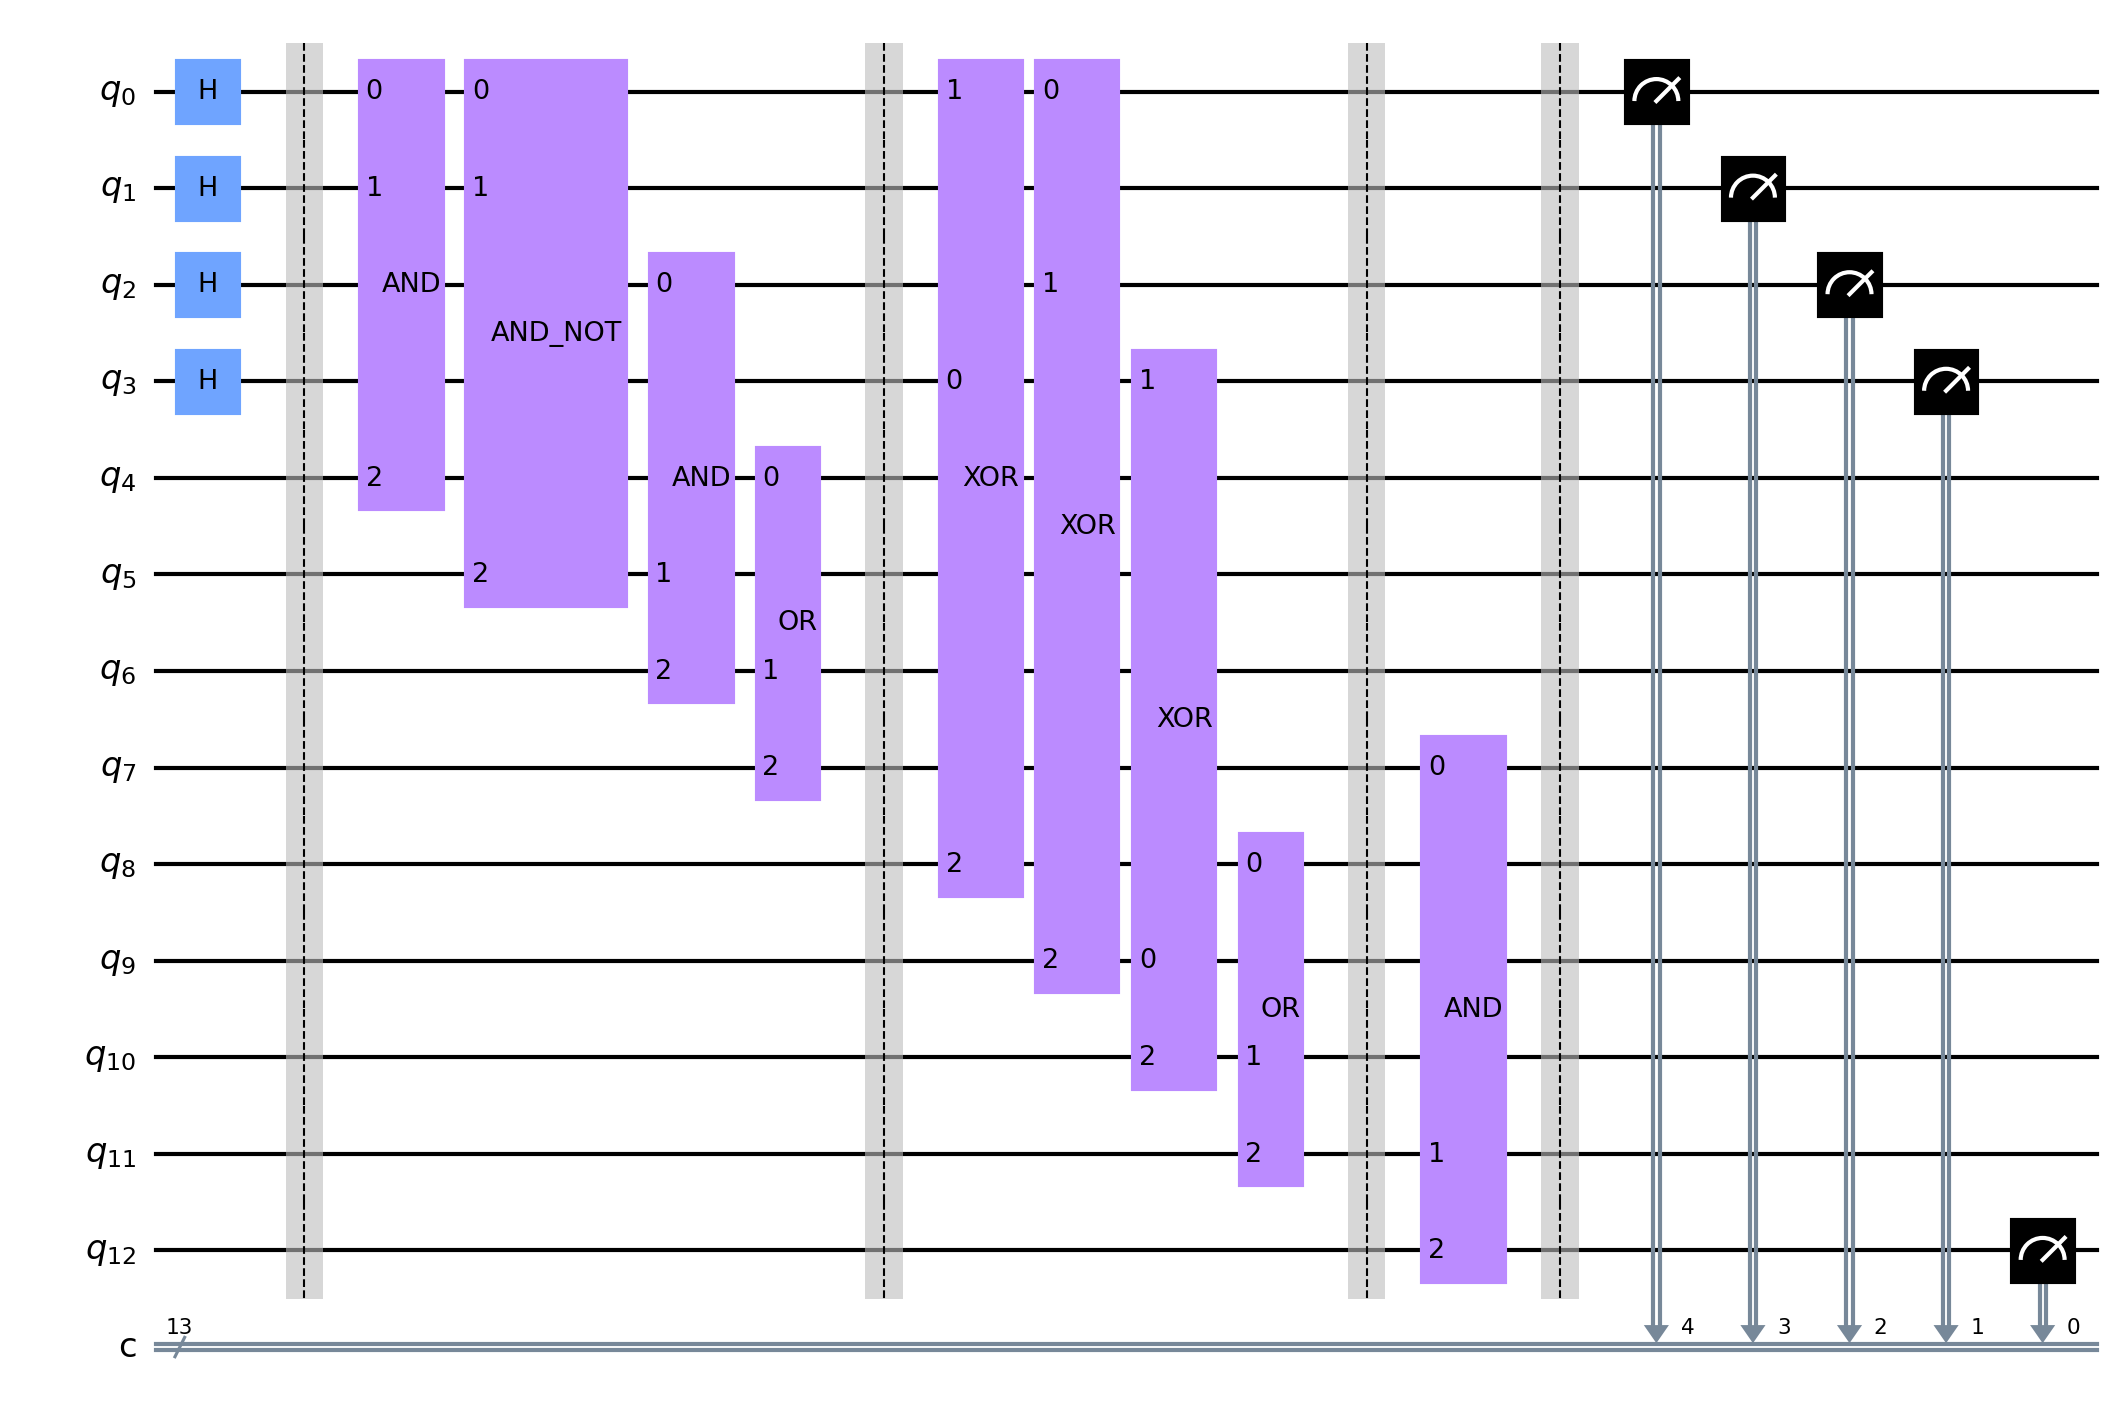
\includegraphics[scale=0.25]{circuit.png}
        }
        \caption{$f(a, b, c, d) = ((a \land b) \lor (a \land \neg b \land c)) \land ((d \oplus a) \lor (a \oplus c \oplus d))$}
        \label{fig:circ_ex_1_1_1}
    \end{figure}
\end{frame}

\section[Problèmes combinatoires]{Optimisation de problèmes combinatoires - Recuit quantique}

\begin{frame}
    \frametitle{Modèle d'Ising}

    \begin{block}{Définition}
        L'énergie d'un système peut être donnée par l'opérateur Hamiltonien. On l'écrit avec le modèle d'Ising de la façon suivante:

        \begin{equation}
            \mathcal{H} = -\displaystyle\sum_{<i, j>} J_{ij} \sigma_i \sigma_j - \displaystyle\sum_{i} h_i \sigma_i .
        \end{equation}

        On a d'un côté le terme $\displaystyle\sum h_i \sigma_i$ indiquant la contribution de chaque variable au système global, c'est le \textbf{biais} du système.

        \hspace{10cm}

        De l'autre côté, on a $\displaystyle\sum J_{ij} \sigma_i \sigma_j$ indiquant les interactions entre chaque paires de variables. C'est le \textbf{couplage} du système.
    \end{block}
\end{frame}

\begin{frame}
    \frametitle{Recuit Quantique}

    Utilisation d'un opérateur Hamiltonien évoluant au cours du temps:

    \begin{equation}
        \mathcal{H}(t) = A(t) \mathcal{H}_0 + B(t) \mathcal{H}_1.
    \end{equation}

    On fait évoluer $A(t)$ de 1 à 0, et $B(t)$ de 0 à 1.
\medbreak
    En prenant un Hamiltonien $\mathcal{H}_0$ tel qu'on puisse construire facilement son état minimal, on fait évoluer le système vers $\mathcal{H}_1$, en restant dans un état minimal du système (théorème adiabatique quantique).

\end{frame}

\begin{frame}[fragile]
    \frametitle{Utilisation de D-Wave - 1}
    Résolution du problème du voyageur de commerce avec les outils fournis par D-Wave:
    \begin{lstlisting}[style=CStyle, basicstyle=\tiny]
import dwave_networkx
import networkx
import dimod
g = networkx.Graph()
g.add_weighted_edges_from({(0, 1, .1), (0, 2, .5), (0, 3, .1), (1, 2, .1),(1, 3, .5), (2, 3, .1)})

dwave_networkx.algorithms.traveling_salesperson(g, dimod.ExactSolver(), start=0)
\end{lstlisting}

\begin{figure}
    \begin{tikzpicture}
        \draw[gray] (-1.25,-0.25) grid[xstep=0.5, ystep=0.5]  (2.25,2.25);
        \node[circle,fill=black,inner sep=0pt,minimum size=3pt,label=below:{\tiny $0$}] (a) at (-1,1) {};
        \node[circle,fill=black,inner sep=0pt,minimum size=3pt,label=above:{\tiny $1$}] (a) at (0.5, 2) {};
        \node[circle,fill=black,inner sep=0pt,minimum size=3pt,label=below:{\tiny $2$}] (a) at (0.5, 0) {};
        \node[circle,fill=black,inner sep=0pt,minimum size=3pt,label=below:{\tiny $3$}] (a) at (2, 1) {};
        \draw (-1,1) -- (0.5, 2)   node [midway,below] {\tiny 0.1};  % 0 - 1
        \draw (-1,1) -- (0.5, 0)   node [midway,below] {\tiny 0.5};  % 0 - 2
        \draw (0.5, 0) -- (0.5, 2) node [pos=0.3,right] {\tiny 0.1}; % 1 - 2
        \draw (0.5, 0) -- (2, 1)   node [midway,below] {\tiny 0.1};  % 2 - 3
        \draw (-1,1) -- (2, 1)     node [pos=0.3,below] {\tiny 0.1}; % 0 - 3
        \draw (0.5, 2) -- (2, 1)   node [midway,below] {\tiny 0.5};  % 1 - 3
    \end{tikzpicture}
    \caption{\tiny Graphe TSP correspondant}
\end{figure}

\end{frame}

\begin{frame}[fragile]
    \frametitle{Utilisation de D-Wave - 2}
    Résolution directe de problème Ising et QUBO: utilisation des solvers D-Wave.
    \begin{lstlisting}[style=CStyle, basicstyle=\tiny]
import dimod
import neal
''' 2 QUBO problems '''
Q1 = {('q1', 'q1'): 0.1, ('q2', 'q2'): 0.1, ('q1', 'q2'): -0.2}
Q2 = {('q1', 'q1'): 0.5, ('q2', 'q2'): 0.5, ('q1', 'q2'): -1}
''' 2 types of solvers: exact, and simulated annealing '''
exact_sampler = dimod.ExactSolver()
sa_sampler = neal.SimulatedAnnealingSampler()
''' Solve using exact solver '''
sample_set = exact_sampler.sample_qubo(Q1)
print(sample_set)
''' Solve using simulated annealing'''
sample_set_1 = exact_sampler.sample_qubo(Q2)
print(sample_set_1)

\end{lstlisting}
\end{frame}

\section[Détection optimale]{Détecteur quantique optimal}

\begin{frame}
\end{frame}

\end{document}